\section{Overview}

Static binary instrumentation generates a modified executable 
 that can be run at a later time. When the instrumented executable is
run, the extra instrumentation code is run
in addition to the original code of the program. In order to insert additional code
and data, additional space must be allocated within the executable in a way that it
will, at load-time, be treated by the system in a manner appropriate to its
purpose. 

Most compilers produce an ELF executable whose
structure is similar to that shown in Figure \ref{Figure:OrigExecutable}. By
convention, most executables use only two loadable segments and some of the Linux
implementations, such as FreeBSD, only allow two loadable segments. Thus, it is
preferable for us to incorporate instrumentation text and data into the
existing text and data segments of the application. The default in most
compilers is to place the text segment prior and adjacent to the data segment.
We therefore prepend the instrumentation text to the existing text
segment\footnote{The amount of space allocated prior to the text section is
controlled by the linker variable \_\_executable\_start. We have seen cases
where the system does not provide enough space prior to the text segment by
default, in which case we provide a set of tools that produces a modified linker
script that provides up to 128MB of space.} and append the instrumentation data to the
data segment (as shown in Figure \ref{Figure:InstExecutable}). This
scheme has the added benefit of causing no immediate disturbance to the
addresses of the existing text and data segments of the program.

\begin{figure}[ht]
\centering
\caption[Optional caption for list of figures]{\subref{Figure:OrigExecutable} and \subref{Figure:InstExecutable} show the prepending
of instrumentation text to the existing text, and the prepending of instrumentation data to the existing data respectively.}
\subfigure[The structure of an unmodified typical ELF file.]{
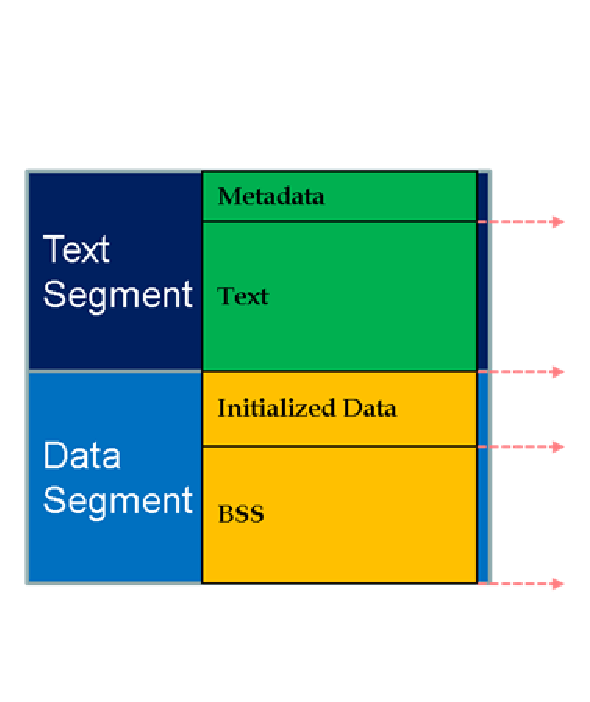
\includegraphics[scale=0.65]{executablep1.eps}
\label{Figure:OrigExecutable}
}
\subfigure[The structure of instrumented ELF file.]{
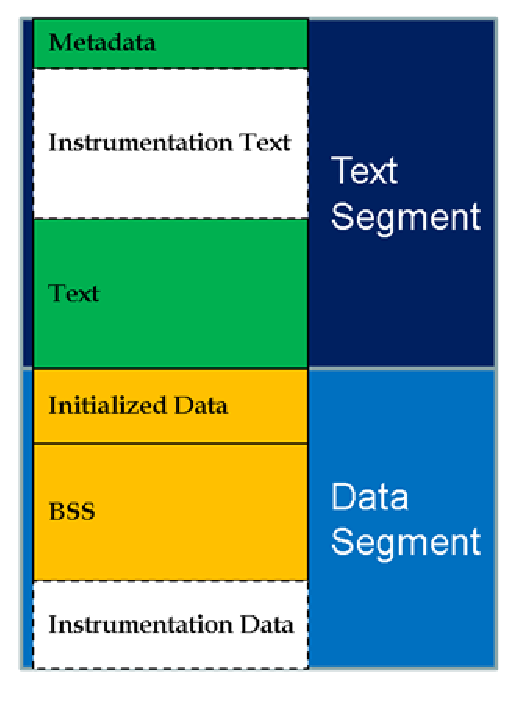
\includegraphics[scale=0.65]{executablep2.eps}
\label{Figure:InstExecutable}
}
\label{Figure:Executable}
\end{figure}

The instrumentation text contains several types of additional code. The first
contains code that accomplishes the instrumentation task as well as some code to
accompany it. When control is transferred from the application to the
instrumentation code, it is necessary to maintain the machine state of
the application in order to preserve its original behavior. This machine state
can contain anything modified by the instrumentation code, but in practice is
usually limited to a relatively limited set of registers but in some cases includes
some information about the call stack. The code snippet, called a \textit{trampoline} \cite{buck2000api}, 
saves any machine state that will be destoryed, performs the instrumentation task, restores
the machine state after the instrumentation, executes the
original instructions that were displaced by the initial control transfer,
finally restoring control to the application. Since we are using a jump instruction at the instrumentation point, the
instrumentation code has no information about where control was transferred from
(as might be the case if we used a more heavyweight call instruction). Hence
each instrumentation point uses its own trampoline so that the location of the
instrumentation point can be hard-coded into an unconditional branch instruction
at the end of the trampoline.

Since some instrumentation tasks may need to include additional data for instrumentation code inserted,
PIX provides mechanisms to add and initialize additional data in to the executable.
The instrumentation text also includes code to initialize this additional data for use by the
instrumentation tool. Recall from Figure \ref{Figure:Executable} that the instrumentation
data was appended to the end of the application's data segment, after the
application's uninitialized data section (BSS section) in order to preserve the application's 
original addresses. The initialized data and BSS
sections of the data segment are usually implemented by declaring the size of
the data segment in the executable to be smaller than the size of the data
segment in memory. According to the ELF specification\cite{standard1995executable}, the extra part of any
segment whose memory size is greater than its file size should be filled with
zeroes by the loader. Hence most programs just increase the size of the data
segment in memory by the size of the BSS section in order to get a large
area that is filled with zeroes and is reserved for uninitialized data. Since we
would like to use the area following the BSS section for additional
data for the instrumentation tool, we can either explicitly include the entire
segment's contents in the executable file or we can implicitly reserve this area
that is already in use by most programs.
Since the BSS section can be very large and explicit inclusion of its contents
would bloat the  executable file, we use the implicit
technique to reserve this section for instrumentation data. We therefore
temporarily store the instrumentation data with the instrumentation text in the
executable, as well as some code to copy it to the appropriate location in the
data segment once the program starts.
